\documentclass[12pt,a4paper]{article}

\usepackage[left=2cm,right=2cm,top=2cm,bottom=2cm]{geometry} % less blank area
\usepackage{amsmath,amssymb,bm,dsfont} % for math
\usepackage{array}   % for eqnarray
\usepackage{arydshln}
\usepackage{graphicx}
\usepackage{enumerate} % for stylish enumrate
\usepackage{listings} % for code demonstration
\usepackage{color}    % for code highlight
\usepackage{fancyhdr} % for header and footnote
\usepackage{lastpage} % for calculating total pages
\usepackage{subfig} % for subfigure
\usepackage{tikz} % for drawing
\usepackage{pdfpages} % for importing PDF files

\newcommand{\docTitle}{IN2106 Practical Course -- Vision-based Navigation: Exercise \#5}
\newcommand{\docSubtitle}{Topic: Backend}
\newcommand{\docAuthor}{Min-An Chao (03681062)}
\newcommand{\docAuthorDept}{TUM MS Informatics}
\newcommand{\docAuthorEmail}{ga83fok@mytum.de}
\newcommand{\docDate}{30.05.2018}

\pagestyle{fancy}
\fancyhf{}
\lhead{\textit{\docTitle}}
\rhead{\textit{\docAuthor}}
\cfoot{\textit{- Page \thepage of \pageref{LastPage} -}}

\lstset{ language={},
         basicstyle=\ttfamily\footnotesize,
         keywordstyle=\color{blue}\ttfamily\footnotesize,
         commentstyle=\color{magenta}\ttfamily\footnotesize,
         morecomment=[l][\color{magenta}\footnotesize]{\#}
}

\setlength{\parindent}{0cm}
\setlength{\parskip}{0.5cm}

% for vector and matrix
\newcommand{\vct}[1]{\boldsymbol{#1}}
\newcommand{\mtx}[1]{\mathbf{#1}}
\newcommand{\set}[1]{\mathcal{#1}}
\newcommand{\dom}[1]{\mathbb{#1}}
\newcommand{\fnc}[1]{\text{#1}}

\DeclareMathOperator*{\argmin}{argmin}
\DeclareMathOperator*{\argmax}{argmax}

% for alignment argument of matrix/pmatrix
\makeatletter
\renewcommand*\env@matrix[1][c]{\hskip -\arraycolsep
  \let\@ifnextchar\new@ifnextchar
  \array{*\c@MaxMatrixCols #1}}
\makeatother

\begin{document}
    \title{\vspace{-1.75cm} \large \textsf{\textbf{\docTitle}}\\ \textsf{\docSubtitle}}
    \author{\normalsize \textsf{
        \textbf{\docAuthor} \hspace{6pt}\textbar\hspace{6pt}
        \docAuthorDept \hspace{6pt}\textbar\hspace{6pt}
        \docAuthorEmail}}
    \date{\small \textsf{\docDate}}
    \maketitle 
    \thispagestyle{fancy}
    \vspace{-0.5cm}
    \hrule
    
    \section{Bundle Adjustment}
    The results are from \texttt{g2o} implementation 
    with \texttt{Ceres} \texttt{AutoDiff} library.
    As shown in Fig.~\ref{fig:bal}, 
    which is from the "Final" set of BAL dataset.
    As we can see after bundle adjustment, 
    the details in the top and the ladder of the building
    are more clear and noisy points reduced.

    \begin{figure}[!ht]
        \centering
        \subfloat[Before BA]{
            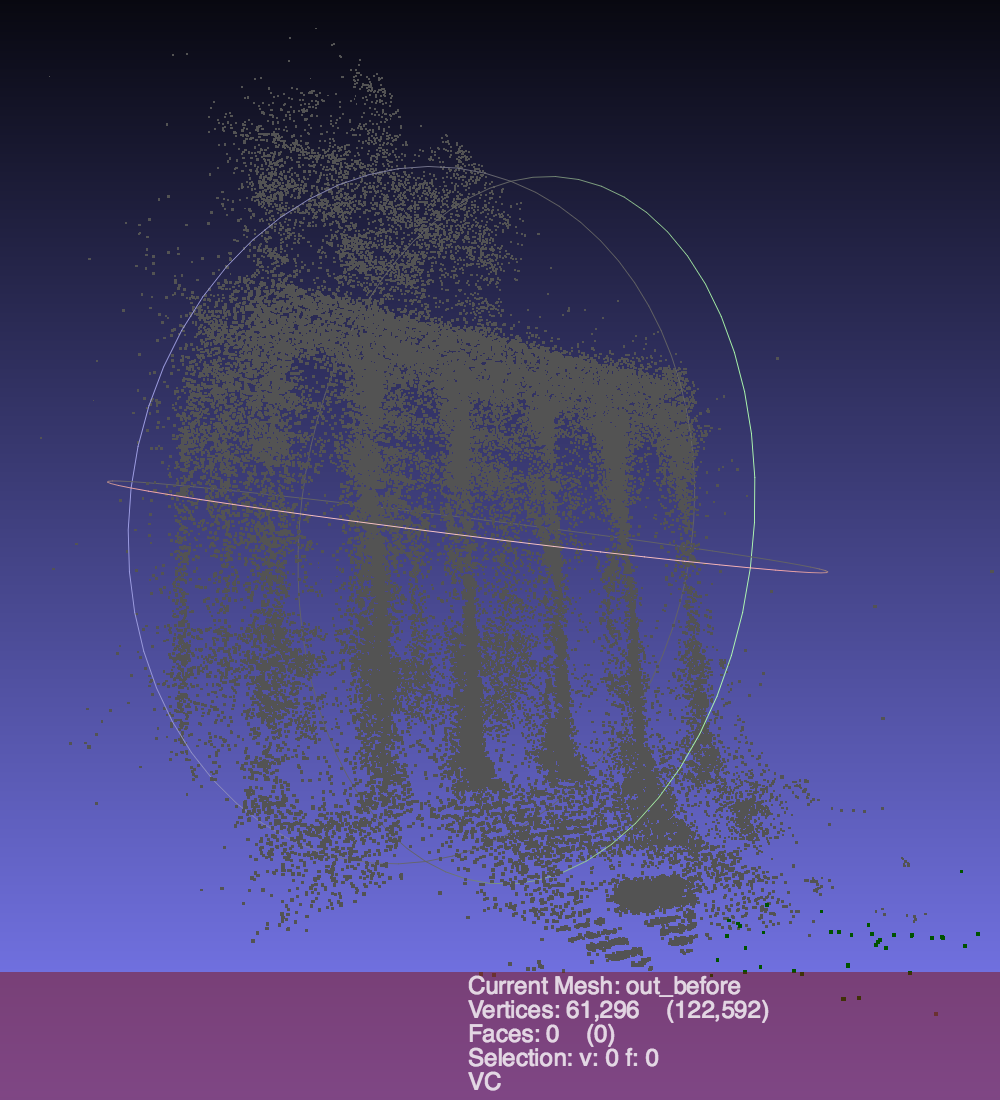
\includegraphics[height=7cm]{fig/bal_before.png}
        }
        \subfloat[After BA]{
            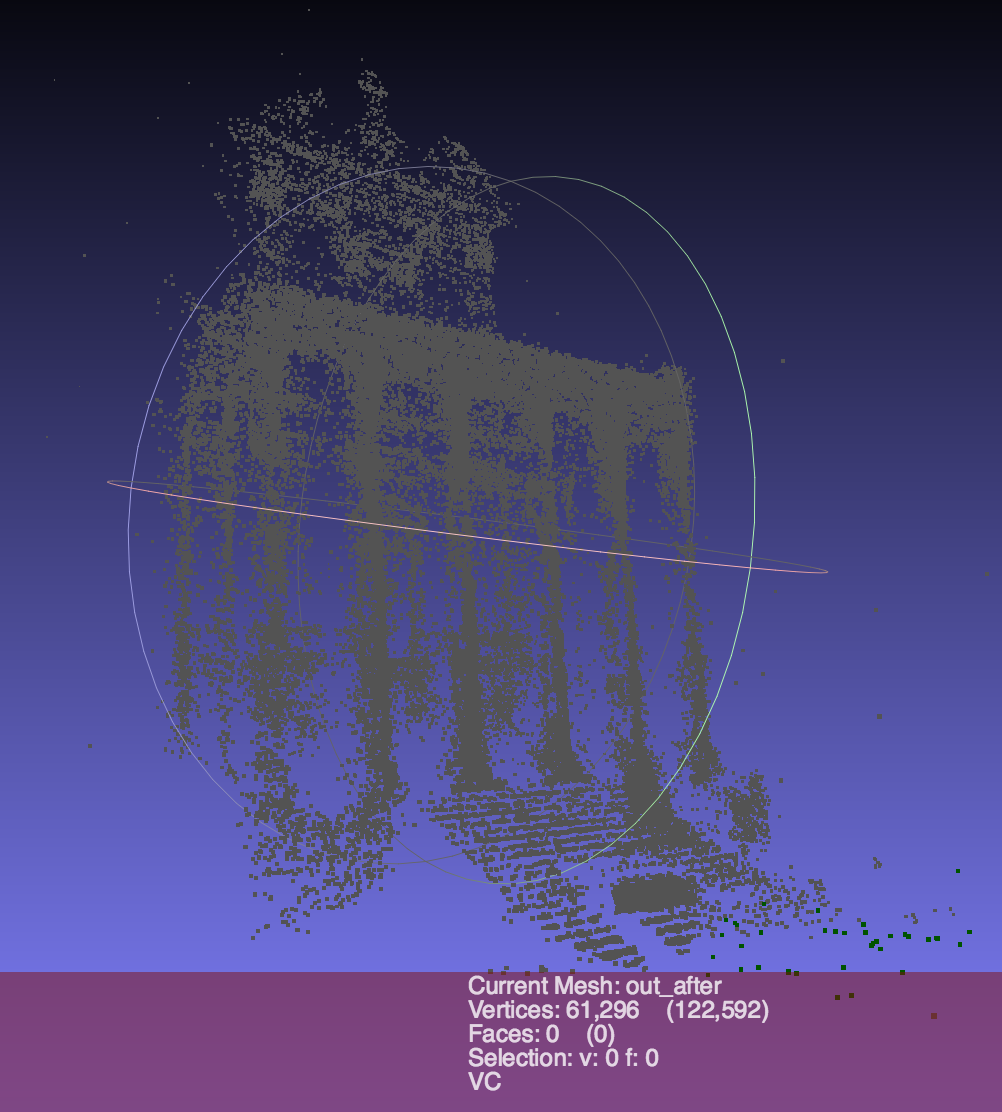
\includegraphics[height=7cm]{fig/bal_after.png}
        }
        \caption{BAL results for "Final" set of BAL dataset}
        \label{fig:bal}
    \end{figure}


    \section{Photometric Bundle Adjustment}
    
    Poses before and after PBA are shown below. 
    Here we just pick camera 0 and camera 6 
    to have a general idea how results are,
    because for these pictures,
    optimization does not really change the points a lot,
    for they are originally good enough.
    Camera 0:
    \begin{lstlisting}[frame=single,numbers=left]
Before optimization:
poses 0: 
   0.92309   0.299879   0.240787   0.702775
 -0.329161    0.93984  0.0913977   0.084358
 -0.198893  -0.163626   0.966265 0.00503326
         0          0          0          1
After optimization:
poses 0: 
  0.923075   0.299655   0.241123   0.702736
 -0.328849   0.940016  0.0907099   0.085861
 -0.199478  -0.163025   0.966246 0.00619912
         0          0          0          1
    \end{lstlisting}
    Camera 6:
    \begin{lstlisting}[frame=single,numbers=left]
Before optimization:
poses 6: 
  0.946979    0.32073 -0.0190444   0.763371
  -0.31505   0.938569   0.140827   0.172428
  0.063042  -0.127361   0.989851  0.0192505
         0          0          0          1
After optimization:
poses 6: 
 0.947043  0.320569 -0.018598  0.763173
-0.314972  0.938655  0.140425  0.172626
 0.062473  -0.12713  0.989917  0.019211
        0         0         0         1
    \end{lstlisting}
    Visual comparison is shown in Fig.~\ref{fig:pba},
    which looks indistinguishable.
    
    \begin{figure}[!ht]
        \centering
        \subfloat[Before PBA]{
            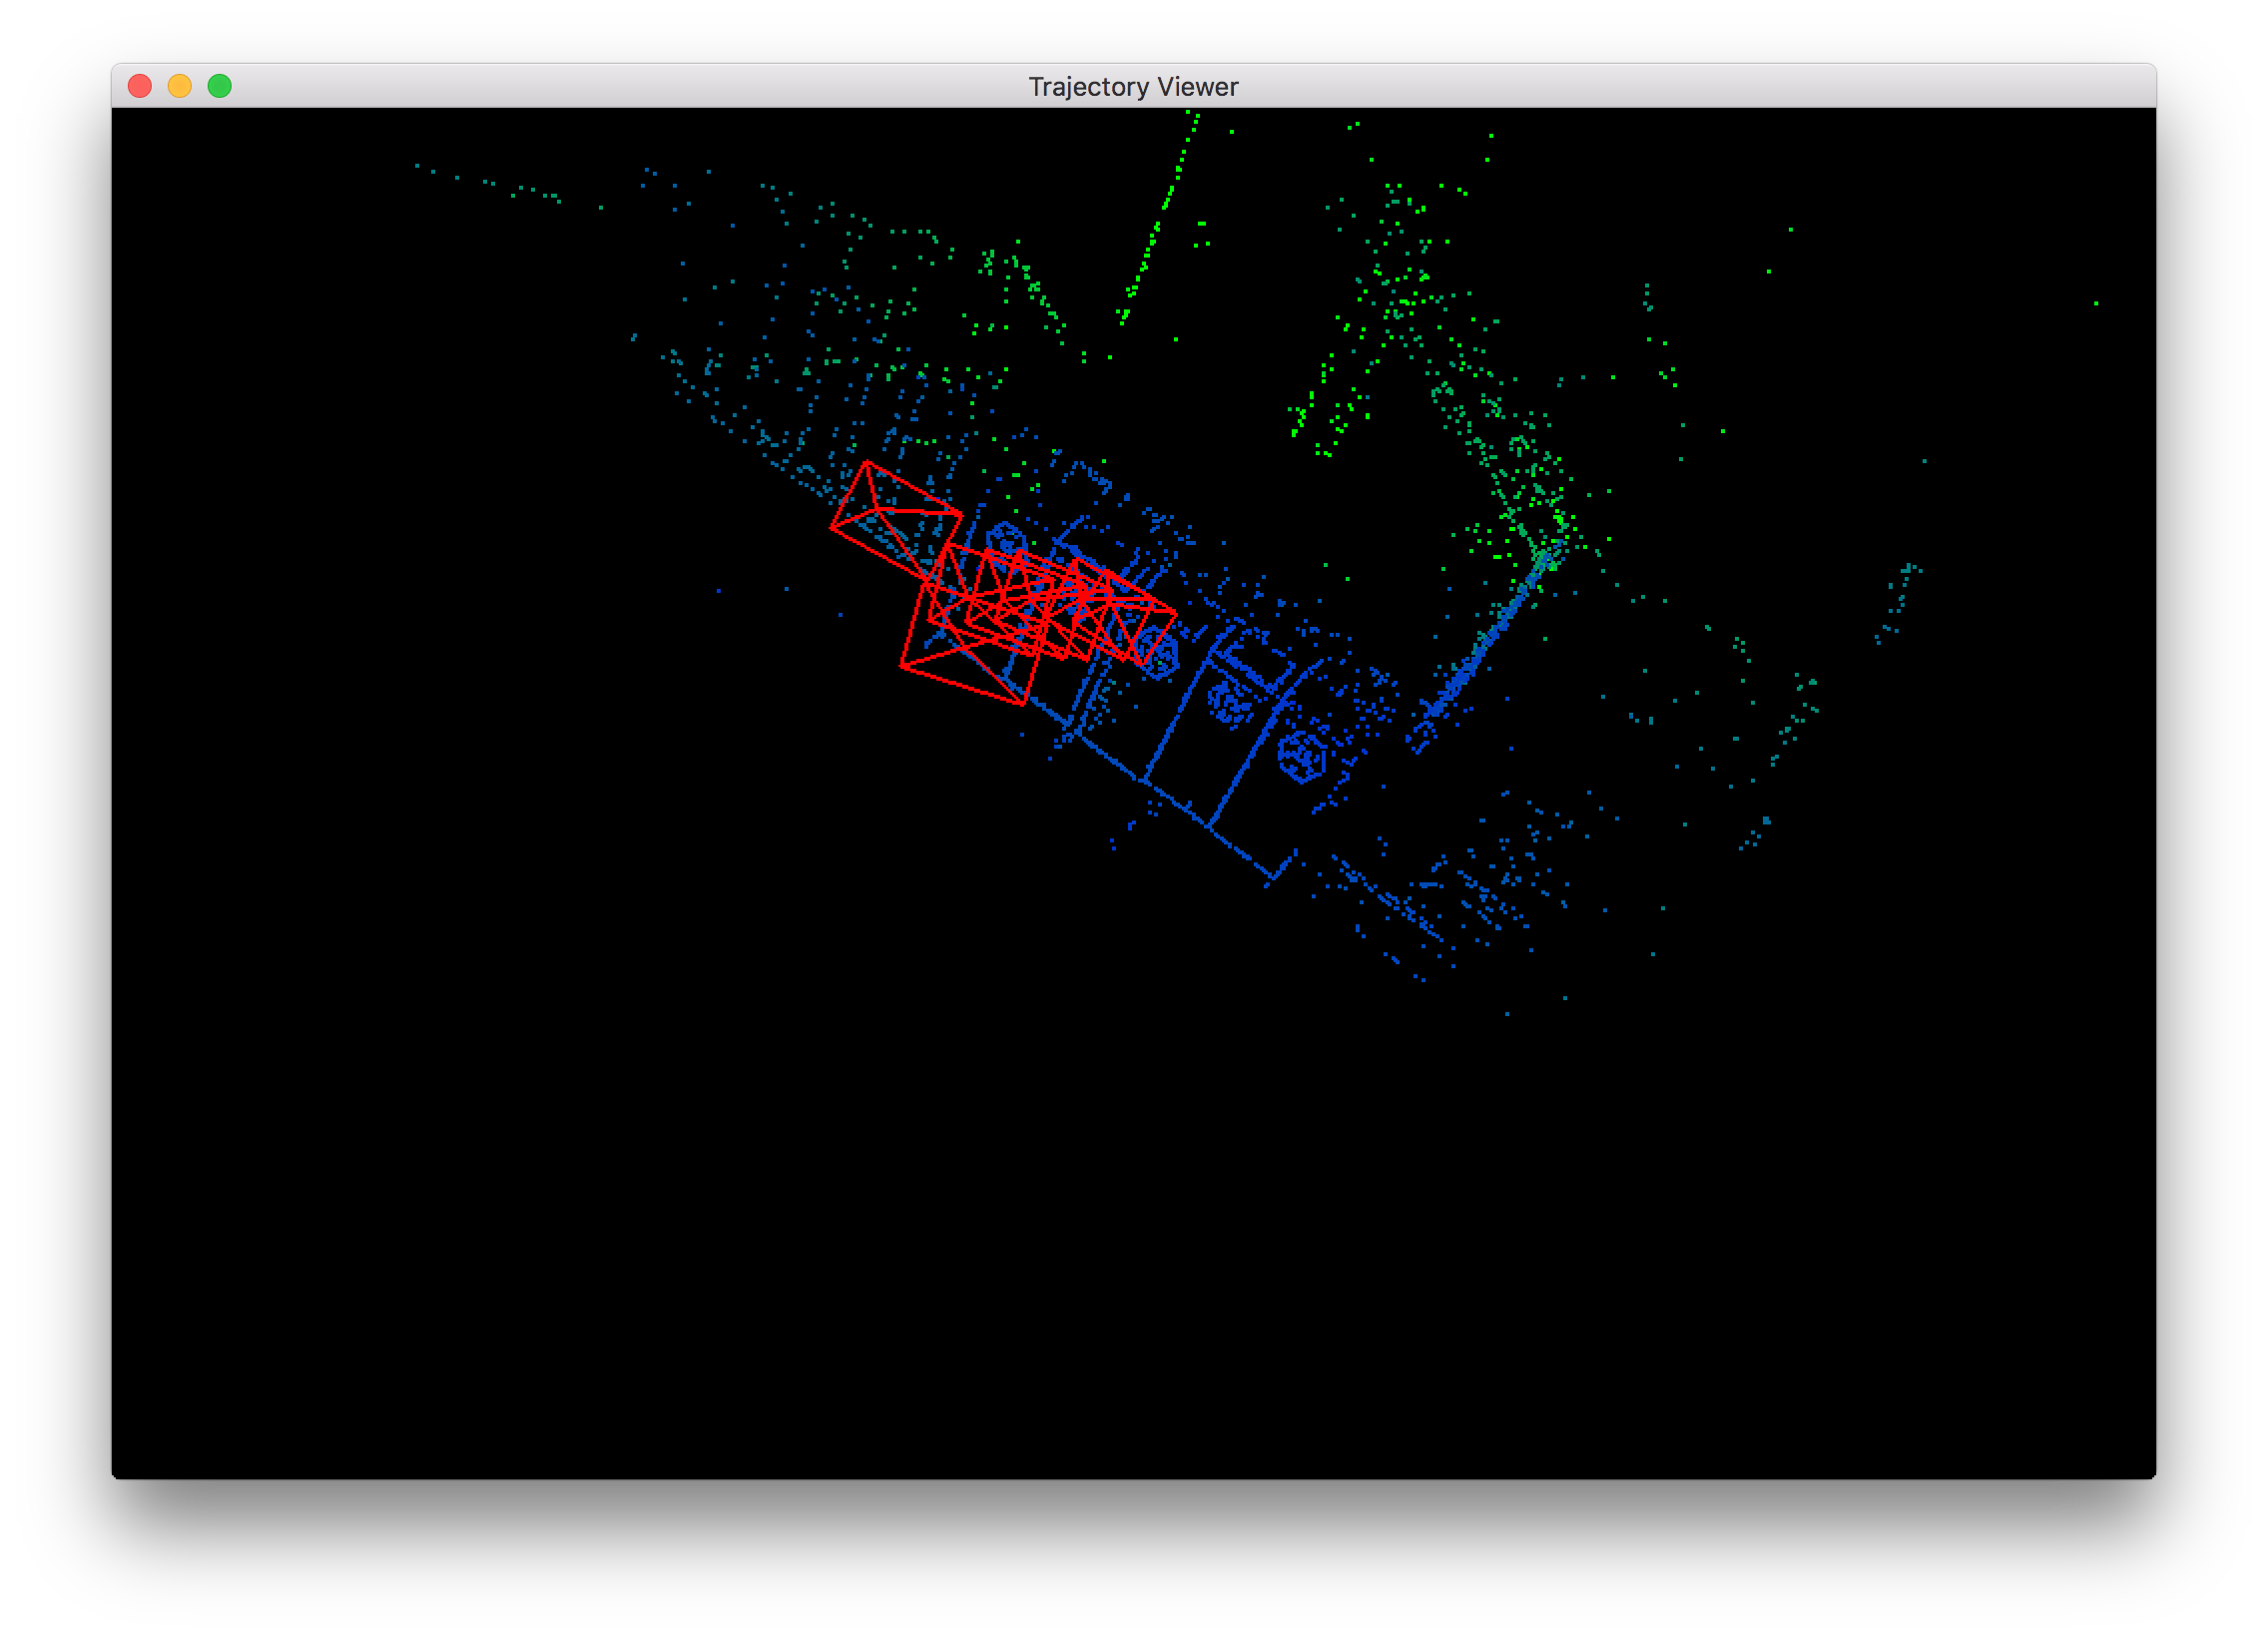
\includegraphics[height=6cm]{fig/pba_before.png}
        }
        \subfloat[After PBA]{
            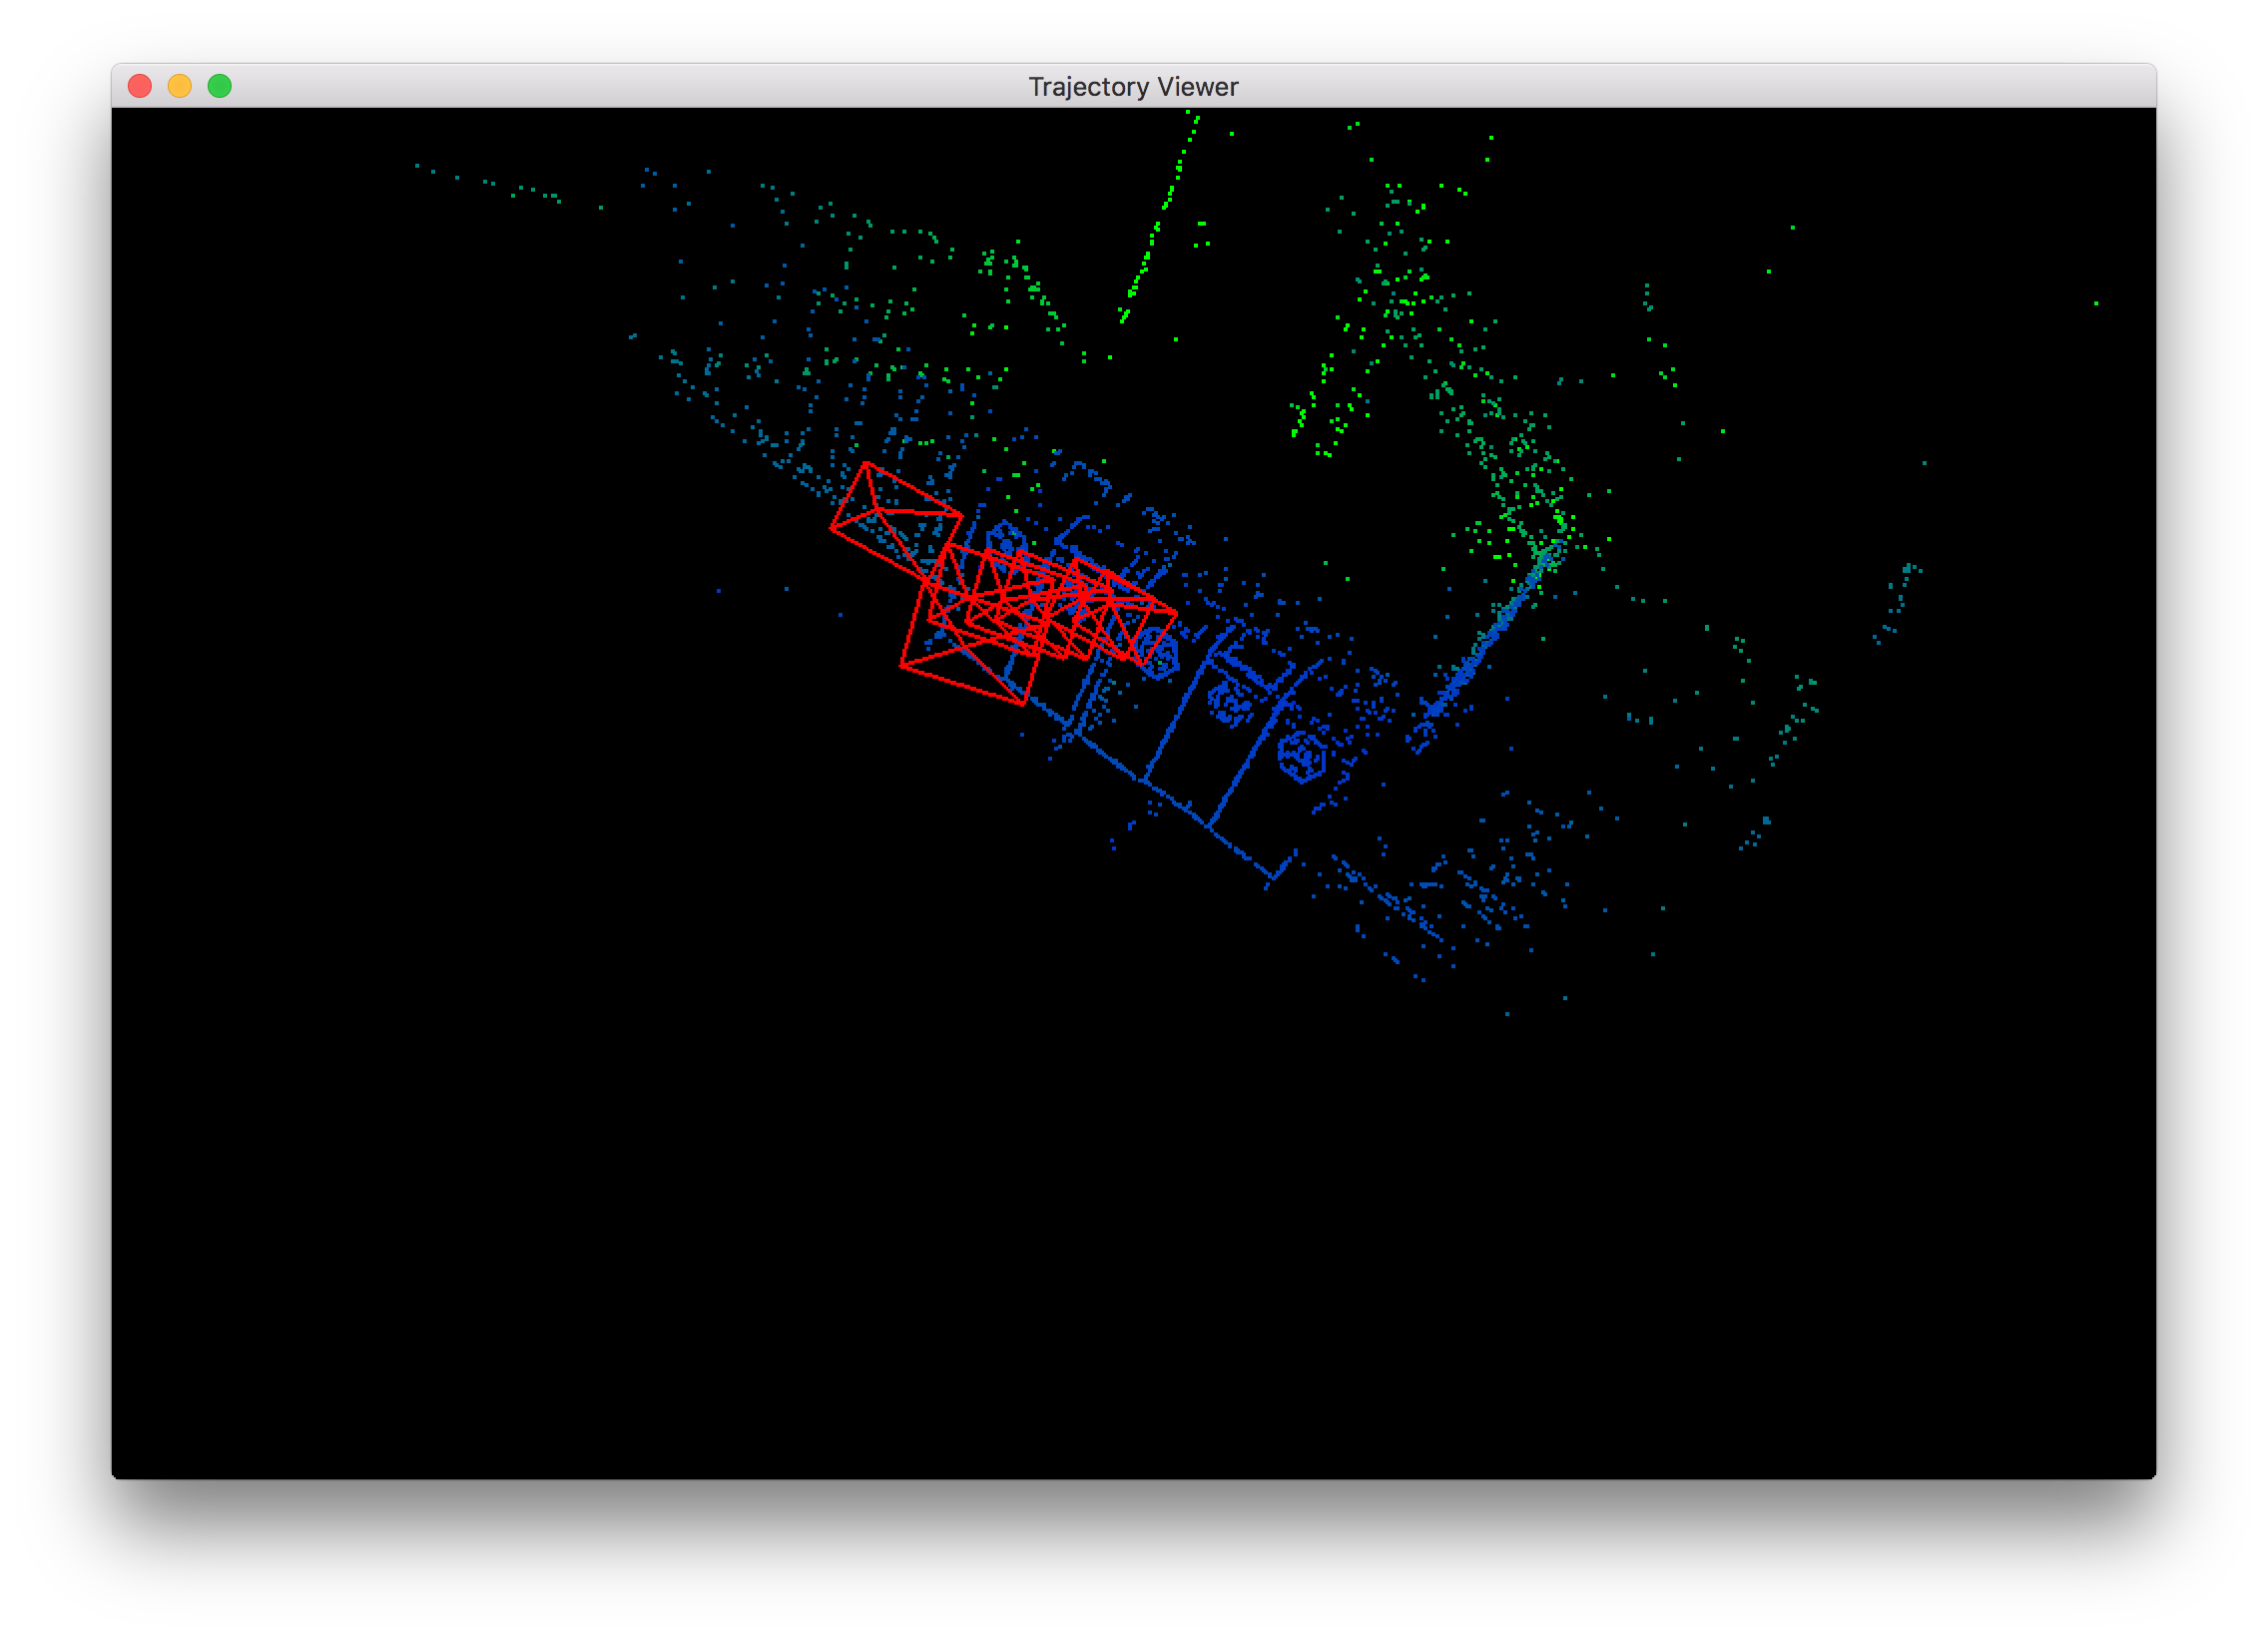
\includegraphics[height=6cm]{fig/pba_after.png}
        }
        \caption{PBA results of given dataset}
        \label{fig:pba}
    \end{figure}

%% template for figures
%   \begin{figure}[!h]
%       \centering
%       \includegraphics[height=6cm]{fig/xxx.png}
%       \caption{XXX}
%       \label{fig:xxx}
%   \end{figure}
%% template for source code or results
%   \begin{lstlisting}[frame=single,numbers=left]
%   \end{lstlisting}
    
\end{document}
